%\documentclass[12pt]{article}
\documentclass[12pt,landscape]{article}

\usepackage[normalem]{ulem}
%packages
%\usepackage{latexsym}
\usepackage{graphicx}
\usepackage{color}
\usepackage{amsmath}
\usepackage{dsfont}
\usepackage{placeins}
\usepackage{amssymb}
\usepackage{wasysym}
\usepackage{abstract}
\usepackage{hyperref}
\usepackage{etoolbox}
\usepackage{datetime}
\usepackage{xcolor}
\usepackage{alphalph}
\settimeformat{ampmtime}

%\usepackage{pstricks,pst-node,pst-tree}

%\usepackage{algpseudocode}
%\usepackage{amsthm}
%\usepackage{hyperref}
%\usepackage{mathrsfs}
%\usepackage{amsfonts}
%\usepackage{bbding}
%\usepackage{listings}
%\usepackage{appendix}
\usepackage[margin=1in]{geometry}
%\geometry{papersize={8.5in,11in},total={6.5in,9in}}
%\usepackage{cancel}
%\usepackage{algorithmic, algorithm}

\makeatletter
\def\maxwidth{ %
  \ifdim\Gin@nat@width>\linewidth
    \linewidth
  \else
    \Gin@nat@width
  \fi
}
\makeatother

\definecolor{fgcolor}{rgb}{0.345, 0.345, 0.345}
\newcommand{\hlnum}[1]{\textcolor[rgb]{0.686,0.059,0.569}{#1}}%
\newcommand{\hlstr}[1]{\textcolor[rgb]{0.192,0.494,0.8}{#1}}%
\newcommand{\hlcom}[1]{\textcolor[rgb]{0.678,0.584,0.686}{\textit{#1}}}%
\newcommand{\hlopt}[1]{\textcolor[rgb]{0,0,0}{#1}}%
\newcommand{\hlstd}[1]{\textcolor[rgb]{0.345,0.345,0.345}{#1}}%
\newcommand{\hlkwa}[1]{\textcolor[rgb]{0.161,0.373,0.58}{\textbf{#1}}}%
\newcommand{\hlkwb}[1]{\textcolor[rgb]{0.69,0.353,0.396}{#1}}%
\newcommand{\hlkwc}[1]{\textcolor[rgb]{0.333,0.667,0.333}{#1}}%
\newcommand{\hlkwd}[1]{\textcolor[rgb]{0.737,0.353,0.396}{\textbf{#1}}}%

\usepackage{framed}
\makeatletter
\newenvironment{kframe}{%
 \def\at@end@of@kframe{}%
 \ifinner\ifhmode%
  \def\at@end@of@kframe{\end{minipage}}%
  \begin{minipage}{\columnwidth}%
 \fi\fi%
 \def\FrameCommand##1{\hskip\@totalleftmargin \hskip-\fboxsep
 \colorbox{shadecolor}{##1}\hskip-\fboxsep
     % There is no \\@totalrightmargin, so:
     \hskip-\linewidth \hskip-\@totalleftmargin \hskip\columnwidth}%
 \MakeFramed {\advance\hsize-\width
   \@totalleftmargin\z@ \linewidth\hsize
   \@setminipage}}%
 {\par\unskip\endMakeFramed%
 \at@end@of@kframe}
\makeatother

\definecolor{shadecolor}{rgb}{.77, .77, .77}
\definecolor{messagecolor}{rgb}{0, 0, 0}
\definecolor{warningcolor}{rgb}{1, 0, 1}
\definecolor{errorcolor}{rgb}{1, 0, 0}
\newenvironment{knitrout}{}{} % an empty environment to be redefined in TeX

\usepackage{alltt}
\usepackage[T1]{fontenc}

\newcommand{\qu}[1]{``#1''}
\newcounter{probnum}
\setcounter{probnum}{1}

%create definition to allow local margin changes
\def\changemargin#1#2{\list{}{\rightmargin#2\leftmargin#1}\item[]}
\let\endchangemargin=\endlist 

%allow equations to span multiple pages
\allowdisplaybreaks

%define colors and color typesetting conveniences
\definecolor{gray}{rgb}{0.5,0.5,0.5}
\definecolor{black}{rgb}{0,0,0}
\definecolor{white}{rgb}{1,1,1}
\definecolor{blue}{rgb}{0.5,0.5,1}
\newcommand{\inblue}[1]{\color{blue}#1 \color{black}}
\definecolor{green}{rgb}{0.133,0.545,0.133}
\newcommand{\ingreen}[1]{\color{green}#1 \color{black}}
\definecolor{yellow}{rgb}{1,1,0}
\newcommand{\inyellow}[1]{\color{yellow}#1 \color{black}}
\definecolor{orange}{rgb}{0.9,0.649,0}
\newcommand{\inorange}[1]{\color{orange}#1 \color{black}}
\definecolor{red}{rgb}{1,0.133,0.133}
\newcommand{\inred}[1]{\color{red}#1 \color{black}}
\definecolor{purple}{rgb}{0.58,0,0.827}
\newcommand{\inpurple}[1]{\color{purple}#1 \color{black}}
\definecolor{backgcode}{rgb}{0.97,0.97,0.8}
\definecolor{Brown}{cmyk}{0,0.81,1,0.60}
\definecolor{OliveGreen}{cmyk}{0.64,0,0.95,0.40}
\definecolor{CadetBlue}{cmyk}{0.62,0.57,0.23,0}

%define new math operators
\DeclareMathOperator*{\argmax}{arg\,max~}
\DeclareMathOperator*{\argmin}{arg\,min~}
\DeclareMathOperator*{\argsup}{arg\,sup~}
\DeclareMathOperator*{\arginf}{arg\,inf~}
\DeclareMathOperator*{\convolution}{\text{\Huge{$\ast$}}}
\newcommand{\infconv}[2]{\convolution^\infty_{#1 = 1} #2}
%true functions

%%%% GENERAL SHORTCUTS

%shortcuts for pure typesetting conveniences
\newcommand{\bv}[1]{\boldsymbol{#1}}

%shortcuts for compound constants
\newcommand{\BetaDistrConst}{\dfrac{\Gamma(\alpha + \beta)}{\Gamma(\alpha)\Gamma(\beta)}}
\newcommand{\NormDistrConst}{\dfrac{1}{\sqrt{2\pi\sigma^2}}}

%shortcuts for conventional symbols
\newcommand{\tsq}{\tau^2}
\newcommand{\tsqh}{\hat{\tau}^2}
\newcommand{\sigsq}{\sigma^2}
\newcommand{\sigsqsq}{\parens{\sigma^2}^2}
\newcommand{\sigsqovern}{\dfrac{\sigsq}{n}}
\newcommand{\tausq}{\tau^2}
\newcommand{\tausqalpha}{\tau^2_\alpha}
\newcommand{\tausqbeta}{\tau^2_\beta}
\newcommand{\tausqsigma}{\tau^2_\sigma}
\newcommand{\betasq}{\beta^2}
\newcommand{\sigsqvec}{\bv{\sigma}^2}
\newcommand{\sigsqhat}{\hat{\sigma}^2}
\newcommand{\sigsqhatmlebayes}{\sigsqhat_{\text{Bayes, MLE}}}
\newcommand{\sigsqhatmle}[1]{\sigsqhat_{#1, \text{MLE}}}
\newcommand{\bSigma}{\bv{\Sigma}}
\newcommand{\bSigmainv}{\bSigma^{-1}}
\newcommand{\thetavec}{\bv{\theta}}
\newcommand{\thetahat}{\hat{\theta}}
\usepackage{accents}
\newlength{\dhatheight}
\newcommand{\doublehat}[1]{%
    \settoheight{\dhatheight}{\ensuremath{\hat{#1}}}%
    \addtolength{\dhatheight}{-0.35ex}%
    \hat{\vphantom{\rule{1pt}{\dhatheight}}%
    \smash{\hat{#1}}}}

\newcommand{\thetahathat}{\doublehat{\theta}}
\newcommand{\thetahatmm}{\hat{\theta}^{\mathrm{MM}}}
\newcommand{\thetahathatmm}{\thetahathat^{\mathrm{MM}}}
\newcommand{\thetahatmle}{\hat{\theta}^{\mathrm{MLE}}}
\newcommand{\thetahathatmle}{\thetahathat^{\mathrm{MLE}}}
\newcommand{\thetavechatmle}{\hat{\thetavec}^{\mathrm{MLE}}}
\newcommand{\muhat}{\hat{\mu}}
\newcommand{\musq}{\mu^2}
\newcommand{\muvec}{\bv{\mu}}
\newcommand{\muhatmle}{\muhat_{\text{MLE}}}
\newcommand{\lambdahat}{\hat{\lambda}}
\newcommand{\lambdahatmle}{\lambdahat_{\text{MLE}}}
\newcommand{\etavec}{\bv{\eta}}
\newcommand{\alphavec}{\bv{\alpha}}
\newcommand{\minimaxdec}{\delta^*_{\mathrm{mm}}}
\newcommand{\ybar}{\bar{y}}
\newcommand{\xbar}{\bar{x}}
\newcommand{\Xbar}{\bar{X}}
\newcommand{\phat}{\hat{p}}
\newcommand{\Phat}{\hat{P}}
\newcommand{\Zbar}{\bar{Z}}
\newcommand{\iid}{~{\buildrel iid \over \sim}~}
\newcommand{\inddist}{~{\buildrel ind \over \sim}~}
\newcommand{\approxdist}{~{\buildrel approx \over \sim}~}
\newcommand{\equalsindist}{~{\buildrel d \over =}~}
\newcommand{\loglik}[1]{\ell\parens{#1}}
\newcommand{\thetahatkminone}{\thetahat^{(k-1)}}
\newcommand{\thetahatkplusone}{\thetahat^{(k+1)}}
\newcommand{\thetahatk}{\thetahat^{(k)}}
\newcommand{\half}{\frac{1}{2}}
\newcommand{\third}{\frac{1}{3}}
\newcommand{\twothirds}{\frac{2}{3}}
\newcommand{\fourth}{\frac{1}{4}}
\newcommand{\fifth}{\frac{1}{5}}
\newcommand{\sixth}{\frac{1}{6}}

%shortcuts for vector and matrix notation
\newcommand{\A}{\bv{A}}
\newcommand{\At}{\A^T}
\newcommand{\Ainv}{\inverse{\A}}
\newcommand{\B}{\bv{B}}
\newcommand{\K}{\bv{K}}
\newcommand{\Kt}{\K^T}
\newcommand{\Kinv}{\inverse{K}}
\newcommand{\Kinvt}{(\Kinv)^T}
\newcommand{\M}{\bv{M}}
\newcommand{\Bt}{\B^T}
\newcommand{\Q}{\bv{Q}}
\newcommand{\Qt}{\Q^T}
\newcommand{\R}{\bv{R}}
\newcommand{\Rt}{\R^T}
\newcommand{\Z}{\bv{Z}}
\newcommand{\X}{\bv{X}}
\newcommand{\Xsub}{\X_{\text{(sub)}}}
\newcommand{\Xsubadj}{\X_{\text{(sub,adj)}}}
\newcommand{\I}{\bv{I}}
\newcommand{\Y}{\bv{Y}}
\newcommand{\T}{\bv{T}}
\newcommand{\sigsqI}{\sigsq\I}
\renewcommand{\P}{\bv{P}}
\newcommand{\Psub}{\P_{\text{(sub)}}}
\newcommand{\Pt}{\P^T}
\newcommand{\Pii}{P_{ii}}
\newcommand{\Pij}{P_{ij}}
\newcommand{\IminP}{(\I-\P)}
\newcommand{\Xt}{\bv{X}^T}
\newcommand{\XtX}{\Xt\X}
\newcommand{\XtXinv}{\parens{\Xt\X}^{-1}}
\newcommand{\XtXinvXt}{\XtXinv\Xt}
\newcommand{\XXtXinvXt}{\X\XtXinvXt}
\newcommand{\x}{\bv{x}}
\newcommand{\p}{\bv{p}}
\newcommand{\onevec}{\bv{1}}
\newcommand{\oneton}{1, \ldots, n}
\newcommand{\yoneton}{y_1, \ldots, y_n}
\newcommand{\yonetonorder}{y_{(1)}, \ldots, y_{(n)}}
\newcommand{\Yoneton}{Y_1, \ldots, Y_n}
\newcommand{\iinoneton}{i \in \braces{\oneton}}
\newcommand{\onetom}{1, \ldots, m}
\newcommand{\jinonetom}{j \in \braces{\onetom}}
\newcommand{\xoneton}{x_1, \ldots, x_n}
\newcommand{\Xoneton}{X_1, \ldots, X_n}
\newcommand{\xt}{\x^T}
\newcommand{\y}{\bv{y}}
\newcommand{\yt}{\y^T}
\renewcommand{\c}{\bv{c}}
\newcommand{\ct}{\c^T}
\newcommand{\tstar}{\bv{t}^*}
\renewcommand{\u}{\bv{u}}
\renewcommand{\v}{\bv{v}}
\renewcommand{\a}{\bv{a}}
\newcommand{\s}{\bv{s}}
\newcommand{\yadj}{\y_{\text{(adj)}}}
\newcommand{\xjadj}{\x_{j\text{(adj)}}}
\newcommand{\xjadjM}{\x_{j \perp M}}
\newcommand{\yhat}{\hat{\y}}
\newcommand{\yhatsub}{\yhat_{\text{(sub)}}}
\newcommand{\yhatstar}{\yhat^*}
\newcommand{\yhatstarnew}{\yhatstar_{\text{new}}}
\newcommand{\z}{\bv{z}}
\newcommand{\zt}{\z^T}
\newcommand{\bb}{\bv{b}}
\newcommand{\bbt}{\bb^T}
\newcommand{\bbeta}{\bv{\beta}}
\newcommand{\beps}{\bv{\epsilon}}
\newcommand{\bepst}{\beps^T}
\newcommand{\e}{\bv{e}}
\newcommand{\Mofy}{\M(\y)}
\newcommand{\KofAlpha}{K(\alpha)}
\newcommand{\ellset}{\mathcal{L}}
\newcommand{\oneminalph}{1-\alpha}
\newcommand{\SSE}{\text{SSE}}
\newcommand{\SSEsub}{\text{SSE}_{\text{(sub)}}}
\newcommand{\MSE}{\text{MSE}}
\newcommand{\RMSE}{\text{RMSE}}
\newcommand{\SSR}{\text{SSR}}
\newcommand{\SST}{\text{SST}}
\newcommand{\JSest}{\delta_{\text{JS}}(\x)}
\newcommand{\Bayesest}{\delta_{\text{Bayes}}(\x)}
\newcommand{\EmpBayesest}{\delta_{\text{EmpBayes}}(\x)}
\newcommand{\BLUPest}{\delta_{\text{BLUP}}}
\newcommand{\MLEest}[1]{\hat{#1}_{\text{MLE}}}

%shortcuts for Linear Algebra stuff (i.e. vectors and matrices)
\newcommand{\twovec}[2]{\bracks{\begin{array}{c} #1 \\ #2 \end{array}}}
\newcommand{\threevec}[3]{\bracks{\begin{array}{c} #1 \\ #2 \\ #3 \end{array}}}
\newcommand{\fivevec}[5]{\bracks{\begin{array}{c} #1 \\ #2 \\ #3 \\ #4 \\ #5 \end{array}}}
\newcommand{\twobytwomat}[4]{\bracks{\begin{array}{cc} #1 & #2 \\ #3 & #4 \end{array}}}
\newcommand{\threebytwomat}[6]{\bracks{\begin{array}{cc} #1 & #2 \\ #3 & #4 \\ #5 & #6 \end{array}}}

%shortcuts for conventional compound symbols
\newcommand{\thetainthetas}{\theta \in \Theta}
\newcommand{\reals}{\mathbb{R}}
\newcommand{\complexes}{\mathbb{C}}
\newcommand{\rationals}{\mathbb{Q}}
\newcommand{\integers}{\mathbb{Z}}
\newcommand{\naturals}{\mathbb{N}}
\newcommand{\forallninN}{~~\forall n \in \naturals}
\newcommand{\forallxinN}[1]{~~\forall #1 \in \reals}
\newcommand{\matrixdims}[2]{\in \reals^{\,#1 \times #2}}
\newcommand{\inRn}[1]{\in \reals^{\,#1}}
\newcommand{\mathimplies}{\quad\Rightarrow\quad}
\newcommand{\mathlogicequiv}{\quad\Leftrightarrow\quad}
\newcommand{\eqncomment}[1]{\quad \text{(#1)}}
\newcommand{\limitn}{\lim_{n \rightarrow \infty}}
\newcommand{\limitN}{\lim_{N \rightarrow \infty}}
\newcommand{\limitd}{\lim_{d \rightarrow \infty}}
\newcommand{\limitt}{\lim_{t \rightarrow \infty}}
\newcommand{\limitsupn}{\limsup_{n \rightarrow \infty}~}
\newcommand{\limitinfn}{\liminf_{n \rightarrow \infty}~}
\newcommand{\limitk}{\lim_{k \rightarrow \infty}}
\newcommand{\limsupn}{\limsup_{n \rightarrow \infty}}
\newcommand{\limsupk}{\limsup_{k \rightarrow \infty}}
\newcommand{\floor}[1]{\left\lfloor #1 \right\rfloor}
\newcommand{\ceil}[1]{\left\lceil #1 \right\rceil}

%shortcuts for environments
\newcommand{\beqn}{\vspace{-0.25cm}\begin{eqnarray*}}
\newcommand{\eeqn}{\end{eqnarray*}}
\newcommand{\bneqn}{\vspace{-0.25cm}\begin{eqnarray}}
\newcommand{\eneqn}{\end{eqnarray}}

%shortcuts for mini environments
\newcommand{\parens}[1]{\left(#1\right)}
\newcommand{\squared}[1]{\parens{#1}^2}
\newcommand{\tothepow}[2]{\parens{#1}^{#2}}
\newcommand{\prob}[1]{\mathbb{P}\parens{#1}}
\newcommand{\cprob}[2]{\prob{#1~|~#2}}
\newcommand{\littleo}[1]{o\parens{#1}}
\newcommand{\bigo}[1]{O\parens{#1}}
\newcommand{\Lp}[1]{\mathbb{L}^{#1}}
\renewcommand{\arcsin}[1]{\text{arcsin}\parens{#1}}
\newcommand{\prodonen}[2]{\bracks{\prod_{#1=1}^n #2}}
\newcommand{\mysum}[4]{\sum_{#1=#2}^{#3} #4}
\newcommand{\sumonen}[2]{\sum_{#1=1}^n #2}
\newcommand{\infsum}[2]{\sum_{#1=1}^\infty #2}
\newcommand{\infprod}[2]{\prod_{#1=1}^\infty #2}
\newcommand{\infunion}[2]{\bigcup_{#1=1}^\infty #2}
\newcommand{\infinter}[2]{\bigcap_{#1=1}^\infty #2}
\newcommand{\infintegral}[2]{\int^\infty_{-\infty} #2 ~\text{d}#1}
\newcommand{\supthetas}[1]{\sup_{\thetainthetas}\braces{#1}}
\newcommand{\bracks}[1]{\left[#1\right]}
\newcommand{\braces}[1]{\left\{#1\right\}}
\newcommand{\set}[1]{\left\{#1\right\}}
\newcommand{\abss}[1]{\left|#1\right|}
\newcommand{\norm}[1]{\left|\left|#1\right|\right|}
\newcommand{\normsq}[1]{\norm{#1}^2}
\newcommand{\inverse}[1]{\parens{#1}^{-1}}
\newcommand{\rowof}[2]{\parens{#1}_{#2\cdot}}

%shortcuts for functionals
\newcommand{\realcomp}[1]{\text{Re}\bracks{#1}}
\newcommand{\imagcomp}[1]{\text{Im}\bracks{#1}}
\newcommand{\range}[1]{\text{range}\bracks{#1}}
\newcommand{\colsp}[1]{\text{colsp}\bracks{#1}}
\newcommand{\rowsp}[1]{\text{rowsp}\bracks{#1}}
\newcommand{\tr}[1]{\text{tr}\bracks{#1}}
\newcommand{\rank}[1]{\text{rank}\bracks{#1}}
\newcommand{\proj}[2]{\text{Proj}_{#1}\bracks{#2}}
\newcommand{\projcolspX}[1]{\text{Proj}_{\colsp{\X}}\bracks{#1}}
\newcommand{\median}[1]{\text{median}\bracks{#1}}
\newcommand{\mean}[1]{\text{mean}\bracks{#1}}
\newcommand{\dime}[1]{\text{dim}\bracks{#1}}
\renewcommand{\det}[1]{\text{det}\bracks{#1}}
\newcommand{\expe}[1]{\mathbb{E}\bracks{#1}}
\newcommand{\expeabs}[1]{\expe{\abss{#1}}}
\newcommand{\expesub}[2]{\mathbb{E}_{#1}\bracks{#2}}
\newcommand{\indic}[1]{\mathds{1}_{#1}}
\newcommand{\var}[1]{\mathbb{V}\text{ar}\bracks{#1}}
\newcommand{\cov}[2]{\mathbb{C}\text{ov}\bracks{#1, #2}}
\newcommand{\skewness}[1]{\mathbb{S}\text{kew}\bracks{#1}}
\newcommand{\corrtwo}[2]{\text{Corr}\bracks{#1, #2}}
\newcommand{\corr}[1]{\text{Corr}\bracks{#1}}
\newcommand{\se}[1]{\mathbb{S}\text{E}\bracks{#1}}
\newcommand{\sd}[1]{\mathbb{S}\text{D}\bracks{#1}}
\newcommand{\seest}[1]{\hat{\mathbb{S}\text{E}}\bracks{#1}}
\newcommand{\bias}[1]{\text{Bias}\bracks{#1}}
\newcommand{\derivop}[2]{\dfrac{\text{d}}{\text{d} #1}\bracks{#2}}
\newcommand{\partialop}[2]{\dfrac{\partial}{\partial #1}\bracks{#2}}
\newcommand{\secpartialop}[2]{\dfrac{\partial^2}{\partial #1^2}\bracks{#2}}
\newcommand{\mixpartialop}[3]{\dfrac{\partial^2}{\partial #1 \partial #2}\bracks{#3}}

%shortcuts for functions
\renewcommand{\exp}[1]{\mathrm{exp}\parens{#1}}
\renewcommand{\cos}[1]{\text{cos}\parens{#1}}
\renewcommand{\sin}[1]{\text{sin}\parens{#1}}
\newcommand{\sign}[1]{\text{sign}\parens{#1}}
\newcommand{\are}[1]{\mathrm{ARE}\parens{#1}}
\newcommand{\natlog}[1]{\ln\parens{#1}}
\newcommand{\oneover}[1]{\frac{1}{#1}}
\newcommand{\overtwo}[1]{\frac{#1}{2}}
\newcommand{\overn}[1]{\frac{#1}{n}}
\newcommand{\oneoversqrt}[1]{\oneover{\sqrt{#1}}}
\newcommand{\sqd}[1]{\parens{#1}^2}
\newcommand{\loss}[1]{\ell\parens{\theta, #1}}
\newcommand{\losstwo}[2]{\ell\parens{#1, #2}}
\newcommand{\cf}{\phi(t)}

%English language specific shortcuts
\newcommand{\ie}{\textit{i.e.} }
\newcommand{\AKA}{\textit{AKA} }
\renewcommand{\iff}{\textit{iff}}
\newcommand{\eg}{\textit{e.g.} }
\newcommand{\st}{\textit{s.t.} }
\newcommand{\wrt}{\textit{w.r.t.} }
\newcommand{\mathst}{~~\text{\st}~~}
\newcommand{\mathand}{~~\text{and}~~}
\newcommand{\ala}{\textit{a la} }
\newcommand{\ppp}{posterior predictive p-value}
\newcommand{\dd}{dataset-to-dataset}

%shortcuts for distribution titles
\newcommand{\logistic}[2]{\mathrm{Logistic}\parens{#1,\,#2}}
\newcommand{\bernoulli}[1]{\mathrm{Bern}\parens{#1}}
\newcommand{\betanot}[2]{\mathrm{Beta}\parens{#1,\,#2}}
\newcommand{\stdbetanot}{\betanot{\alpha}{\beta}}
\newcommand{\multnormnot}[3]{\mathcal{N}_{#1}\parens{#2,\,#3}}
\newcommand{\normnot}[2]{\mathcal{N}\parens{#1,\,#2}}
\newcommand{\classicnormnot}{\normnot{\mu}{\sigsq}}
\newcommand{\stdnormnot}{\normnot{0}{1}}
\newcommand{\uniformdiscrete}[1]{\mathrm{Uniform}\parens{\braces{#1}}}
\newcommand{\uniform}[2]{\mathrm{U}\parens{#1,\,#2}}
\newcommand{\stduniform}{\uniform{0}{1}}
\newcommand{\geometric}[1]{\mathrm{Geometric}\parens{#1}}
\newcommand{\hypergeometric}[3]{\mathrm{Hypergeometric}\parens{#1,\,#2,\,#3}}
\newcommand{\exponential}[1]{\mathrm{Exp}\parens{#1}}
\newcommand{\gammadist}[2]{\mathrm{Gamma}\parens{#1, #2}}
\newcommand{\poisson}[1]{\mathrm{Poisson}\parens{#1}}
\newcommand{\binomial}[2]{\mathrm{Binomial}\parens{#1,\,#2}}
\newcommand{\negbin}[2]{\mathrm{NegBin}\parens{#1,\,#2}}
\newcommand{\rayleigh}[1]{\mathrm{Rayleigh}\parens{#1}}
\newcommand{\multinomial}[2]{\mathrm{Multinomial}\parens{#1,\,#2}}
\newcommand{\gammanot}[2]{\mathrm{Gamma}\parens{#1,\,#2}}
\newcommand{\cauchynot}[2]{\text{Cauchy}\parens{#1,\,#2}}
\newcommand{\invchisqnot}[1]{\text{Inv}\chisq{#1}}
\newcommand{\invscaledchisqnot}[2]{\text{ScaledInv}\ncchisq{#1}{#2}}
\newcommand{\invgammanot}[2]{\text{InvGamma}\parens{#1,\,#2}}
\newcommand{\chisq}[1]{\chi^2_{#1}}
\newcommand{\ncchisq}[2]{\chi^2_{#1}\parens{#2}}
\newcommand{\ncF}[3]{F_{#1,#2}\parens{#3}}

%shortcuts for PDF's of common distributions
\newcommand{\logisticpdf}[3]{\oneover{#3}\dfrac{\exp{-\dfrac{#1 - #2}{#3}}}{\parens{1+\exp{-\dfrac{#1 - #2}{#3}}}^2}}
\newcommand{\betapdf}[3]{\dfrac{\Gamma(#2 + #3)}{\Gamma(#2)\Gamma(#3)}#1^{#2-1} (1-#1)^{#3-1}}
\newcommand{\normpdf}[3]{\frac{1}{\sqrt{2\pi#3}}\exp{-\frac{1}{2#3}(#1 - #2)^2}}
\newcommand{\normpdfvarone}[2]{\dfrac{1}{\sqrt{2\pi}}e^{-\half(#1 - #2)^2}}
\newcommand{\chisqpdf}[2]{\dfrac{1}{2^{#2/2}\Gamma(#2/2)}\; {#1}^{#2/2-1} e^{-#1/2}}
\newcommand{\invchisqpdf}[2]{\dfrac{2^{-\overtwo{#1}}}{\Gamma(#2/2)}\,{#1}^{-\overtwo{#2}-1}  e^{-\oneover{2 #1}}}
\newcommand{\exponentialpdf}[2]{#2\exp{-#2#1}}
\newcommand{\poissonpdf}[2]{\dfrac{e^{-#1} #1^{#2}}{#2!}}
\newcommand{\binomialpdf}[3]{\binom{#2}{#1}#3^{#1}(1-#3)^{#2-#1}}
\newcommand{\rayleighpdf}[2]{\dfrac{#1}{#2^2}\exp{-\dfrac{#1^2}{2 #2^2}}}
\newcommand{\gammapdf}[3]{\dfrac{#3^#2}{\Gamma\parens{#2}}#1^{#2-1}\exp{-#3 #1}}
\newcommand{\cauchypdf}[3]{\oneover{\pi} \dfrac{#3}{\parens{#1-#2}^2 + #3^2}}
\newcommand{\Gammaf}[1]{\Gamma\parens{#1}}

%shortcuts for miscellaneous typesetting conveniences
\newcommand{\notesref}[1]{\marginpar{\color{gray}\tt #1\color{black}}}

%%%% DOMAIN-SPECIFIC SHORTCUTS

%Real analysis related shortcuts
\newcommand{\zeroonecl}{\bracks{0,1}}
\newcommand{\forallepsgrzero}{\forall \epsilon > 0~~}
\newcommand{\lessthaneps}{< \epsilon}
\newcommand{\fraccomp}[1]{\text{frac}\bracks{#1}}

%Bayesian related shortcuts
\newcommand{\yrep}{y^{\text{rep}}}
\newcommand{\yrepisq}{(\yrep_i)^2}
\newcommand{\yrepvec}{\bv{y}^{\text{rep}}}


%Probability shortcuts
\newcommand{\SigField}{\mathcal{F}}
\newcommand{\ProbMap}{\mathcal{P}}
\newcommand{\probtrinity}{\parens{\Omega, \SigField, \ProbMap}}
\newcommand{\convp}{~{\buildrel p \over \rightarrow}~}
\newcommand{\convLp}[1]{~{\buildrel \Lp{#1} \over \rightarrow}~}
\newcommand{\nconvp}{~{\buildrel p \over \nrightarrow}~}
\newcommand{\convae}{~{\buildrel a.e. \over \longrightarrow}~}
\newcommand{\convau}{~{\buildrel a.u. \over \longrightarrow}~}
\newcommand{\nconvau}{~{\buildrel a.u. \over \nrightarrow}~}
\newcommand{\nconvae}{~{\buildrel a.e. \over \nrightarrow}~}
\newcommand{\convd}{~{\buildrel d \over \rightarrow}~}
\newcommand{\nconvd}{~{\buildrel d \over \nrightarrow}~}
\newcommand{\withprob}{~~\text{w.p.}~~}
\newcommand{\io}{~~\text{i.o.}}

\newcommand{\Acl}{\bar{A}}
\newcommand{\ENcl}{\bar{E}_N}
\newcommand{\diam}[1]{\text{diam}\parens{#1}}

\newcommand{\taua}{\tau_a}

\newcommand{\myint}[4]{\int_{#2}^{#3} #4 \,\text{d}#1}
\newcommand{\laplacet}[1]{\mathscr{L}\bracks{#1}}
\newcommand{\laplaceinvt}[1]{\mathscr{L}^{-1}\bracks{#1}}
\renewcommand{\min}[1]{\text{min}\braces{#1}}
\renewcommand{\max}[1]{\text{max}\braces{#1}}

\newcommand{\Vbar}[1]{\bar{V}\parens{#1}}
\newcommand{\expnegrtau}{\exp{-r\tau}}

%%% problem typesetting
\definecolor{darkgrey}{rgb}{0.10,0.10,0.9}

\newcommand{\problem}[1]{\noindent \colorbox{black}{{\color{yellow} \large{\textsf{\textbf{Problem \arabic{probnum}}}}~}} \addtocounter{probnum}{1} \vspace{0.2cm} \\ \iftoggle{professormode}{}{\color{darkgrey}} #1}

\newcommand{\easysubproblem}[1]{\ingreen{\item} \iftoggle{professormode}{}{\color{darkgrey}} [easy] #1 \color{black} }
\newcommand{\intermediatesubproblem}[1]{\inorange{\item} \iftoggle{professormode}{}{\color{darkgrey}} [harder] #1 \color{black} }
\newcommand{\hardsubproblem}[1]{\inred{\item} \iftoggle{professormode}{}{\color{darkgrey}} [difficult] #1 \color{black} }
\newcommand{\extracreditsubproblem}[1]{\inpurple{\item} \iftoggle{professormode}{}{\color{darkgrey}} [E.C.] #1 \color{black} }


\newcommand{\spc}[1]{\iftoggle{professormode}{\\ \vspace{#1cm}}{\\ \vspace{-0.3cm}}}

\makeatletter
\newalphalph{\alphmult}[mult]{\@alph}{26}
\renewcommand{\labelenumi}{(\alphmult{\value{enumi}})}

\newcommand{\support}[1]{\text{Supp}\bracks{#1}}
\newcommand{\mode}[1]{\text{Mode}\bracks{#1}}
\newcommand{\IQR}[1]{\text{IQR}\bracks{#1}}
\newcommand{\quantile}[2]{\text{Quantile}\bracks{#1,\,#2}}


\newcommand{\instr}{\small Your answer will consist of a lowercase string (e.g. \texttt{aebgd}) where the order of the letters does not matter. \normalsize}

\title{Math 369 / 690 Fall \the\year{} \\ Final Examination}
\author{Professor Adam Kapelner}

\date{Thursday, December 16, \the\year{}}

\begin{document}
\maketitle

%\noindent Full Name \line(1,0){410}

\thispagestyle{empty}

\section*{Code of Academic Integrity}

\footnotesize
Since the college is an academic community, its fundamental purpose is the pursuit of knowledge. Essential to the success of this educational mission is a commitment to the principles of academic integrity. Every member of the college community is responsible for upholding the highest standards of honesty at all times. Students, as members of the community, are also responsible for adhering to the principles and spirit of the following Code of Academic Integrity.

Activities that have the effect or intention of interfering with education, pursuit of knowledge, or fair evaluation of a student's performance are prohibited. Examples of such activities include but are not limited to the following definitions:

\paragraph{Cheating} Using or attempting to use unauthorized assistance, material, or study aids in examinations or other academic work or preventing, or attempting to prevent, another from using authorized assistance, material, or study aids. Example: using an unauthorized cheat sheet in a quiz or exam, altering a graded exam and resubmitting it for a better grade, etc.
\\

\noindent By taking this exam, you acknowledge and agree to uphold this Code of Academic Integrity. \\

%\begin{center}
%\line(1,0){250} ~~~ \line(1,0){100}\\
%~~~~~~~~~~~~~~~~~~~~~signature~~~~~~~~~~~~~~~~~~~~~~~~~~~~~~~~~~~~~~~~~~~~~ date
%\end{center}

\normalsize
\vspace{-0.3cm}
\section*{Instructions}
This exam is 110 minutes (variable time per question) and closed-book. You are allowed \textbf{three} page (front and back) of a \qu{cheat sheet}, blank scrap paper and a graphing calculator. Please read the questions carefully. I recommend answering all questions that are easy first and then circling back to work on the harder ones. \ingray{Gray text} means the text is repeated verbatim from a previous problem. No food is allowed, only drinks. %If the question reads \qu{compute,} this means the solution will be a number otherwise you can leave the answer in \textit{any} widely accepted mathematical notation which could be resolved to an exact or approximate number with the use of a computer. I advise you to skip problems marked \qu{[Extra Credit]} until you have finished the other questions on the exam, then loop back and plug in all the holes. I also advise you to use pencil. The exam is 100 points total plus extra credit. Partial credit will be granted for incomplete answers on most of the questions. \fbox{Box} in your final answers. Good luck!

\pagebreak

%%%%%%%%%%%%%%%%%%%%%%%%%%%%%%%
\problem\timedsection{13} \href{https://en.wikipedia.org/wiki/Benford\%27s_law}{Benford's law} discovered in 1938 a discrete parameterless probability distribution on the first digits of numbers. It is also called the \qu{first-digit law} and was discovered by examining real-world datasets. In real-world datasets, numbers beginning with a 1 are about twice as likely as numbers beginning with a 2. Numbers beginning with a 2 are about 50\% more likely that numbers beginning with a 3, etc. This is especially true in domains such as accounting and taxes. This distribution is used frequently to prove that a dataset is fraudulent i.e. if someone is trying to cheat on their taxes by randomly generating numeric values, their values will not follow Benford's law since most crooks aren't too careful about learning probability theory. Below is the Benford Law distribution's PMF and CDF. It's mean is 3.441.

\begin{table}[h]
\centering
\begin{tabular}{l|lllllllll}
$x$		&	1		& 	2		&	3		&	4		&	5		&	6		&	7		&		8	&	9 \\ \hline
$p(x)$	&	.301	&	.176	&	.125	&	.097	&	.079	&	.067	&	.058	& 		.051	&	.046 \\
$F(x)$  &   .301		&	.477	&	.602	&	.699	&	.778	&	.845	&	.903	& 		.954	&	1.000 \\
\end{tabular}
\end{table}
\FloatBarrier
\vspace{-0.2cm}
\noindent Consider a tax return with $n=45$ numbers. We examine the first digit of the numbers and sort the data. It turns out the first digit is exactly uniformly distributed across all digits i.e. $\x = <1,1,1,1,1,2,2,2,2,2, \ldots, 9,9,9,9,9>$.  This smells of fraud; we will investigate. To test cheating we can use ...

\vspace{-0.1cm}\benum\truefalsesubquestionwithpoints{13} 
\begin{enumerate}[(a)]
\item ... the one sample asymptotic $z$ test for the mean
\item ... the one sample asymptotic $t$ test for the mean
\item ... the one sample Wald test for the mean
\item ... the score test for the mean
\item ... the likelihood ratio test for the mean
\item ... a generalized likelihood ratio test
\item ... Pearson's $\chi^2$ goodness of fit test
\item ... Kolmogorov-Smirnov's one-sample test
\item ... a bootstrap test where $\xbar$ is calculated for each bootstrap sample
\item ... the Welch-Satterthwaite $t$ test
\item ... Kolmogorov-Smirnov's two-sample test
\item ... Fisher's two-sample permutation test
\item ... the multivariate delta method
\end{enumerate}
\eenum\instr\pagebreak

%%%%%%%%%%%%%%%%%%%%%%%%%%%%%%%
\problem\timedsection{14} \ingray{\small{\href{https://en.wikipedia.org/wiki/Benford\%27s_law}{Benford's law} discovered in 1938 a discrete parameterless probability distribution on the first digits of numbers. It is also called the \qu{first-digit law} and was discovered by examining real-world datasets. In real-world datasets, numbers beginning with a 1 are about twice as likely as numbers beginning with a 2. Numbers beginning with a 2 are about 50\% more likely that numbers beginning with a 3, etc. This is especially true in domains such as accounting and taxes. This distribution is used frequently to prove that a dataset is fraudulent i.e. if someone is trying to cheat on their taxes by randomly generating numeric values, their values will not follow Benford's law since most crooks aren't too careful about learning probability theory. Below is the distribution's PMF and CDF. It's mean is 3.441.} \normalsize


\vspace{-0.2cm}
\begin{table}[h]
\centering\ingray{
\begin{tabular}{l|lllllllll}

$x$		&	1		& 	2		&	3		&	4		&	5		&	6		&	7		&		8	&	9 \\ \hline
$p(x)$	&	.301	&	.176	&	.125	&	.097	&	.079	&	.067	&	.058	& 		.051	&	.046 \\
$F(x)$  &   .301		&	.477	&	.602	&	.699	&	.778	&	.845	&	.903	& 		.954	&	1.000 \\
\end{tabular}}
\end{table}
\FloatBarrier

\vspace{-0.3cm}
\noindent Consider a tax return with $n=45$ numbers. We examine the first digit of the numbers and sort the data. It turns out the first digit is exactly uniformly distributed across all digits i.e. $\x = <1,1,1,1,1,2,2,2,2,2, \ldots, 9,9,9,9,9>$. This smells of fraud; we will investigate.} To do so, we will employ Pearson's $\chi^2$ goodness of fit test at $\alpha = 5\%$. Critical values you may need to reference are: $F_{\chisq{7}}(14.1) = F_{\chisq{8}}(15.5) = F_{\chisq{9}}(16.9) = F_{\chisq{10}}(18.3) = .95$.

\vspace{-0.2cm}\benum\truefalsesubquestionwithpoints{12} 
\begin{enumerate}[(a)]
\item $H_0: \theta = 3.441$ where $\theta$ denotes the mean of the DGP that generated $x_1, \ldots, x_{45}$
\item $H_0:$ the DGP that generated $x_1, \ldots, x_{45}$ is Benford's law
\item $H_0:$ the PMF of the DGP that generated $x_1, \ldots, x_{45}$ is the $p(x)$ given as $p(x)$ in the table above
%\item $H_0:$ the CDF of the DGP that generated $x_1, \ldots, x_{45}$ is the $p(x)$ given as $F(x)$ in the table above
\item Pearson's $\chi^2$ goodness of fit test statistic is a realization from an approximate $\chisq{7}$ distribution
\item Pearson's $\chi^2$ goodness of fit test statistic is a realization from an approximate $\chisq{9}$ distribution

\item Pearson's $\chi^2$ goodness of fit test statistic is 0
\item Pearson's $\chi^2$ goodness of fit test statistic is 18.05 rounded to the nearest two digits
\item Pearson's $\chi^2$ goodness of fit test statistic is 18.39 rounded to the nearest two digits
\item Pearson's $\chi^2$ goodness of fit test statistic is 213.01 rounded to the nearest two digits
%\item Pearson's $\chi^2$ goodness of fit test statistic is 4888.37 rounded to the nearest two digits
\item Pearson's $\chi^2$ goodness of fit test statistic cannot be computed given the information available

\item $H_0$ is rejected
\item There is sufficient evidence to conclude this person is cheating on their tax return
\end{enumerate}
\eenum\instr\pagebreak

%%%%%%%%%%%%%%%%%%%%%%%%%%%%%%%
\problem\timedsection{13} \ingray{\footnotesize{\href{https://en.wikipedia.org/wiki/Benford\%27s_law}{Benford's law} discovered in 1938 a discrete parameterless probability distribution on the first digits of numbers. It is also called the \qu{first-digit law} and was discovered by examining real-world datasets. In real-world datasets, numbers beginning with a 1 are about twice as likely as numbers beginning with a 2. Numbers beginning with a 2 are about 50\% more likely that numbers beginning with a 3, etc. This is especially true in domains such as accounting and taxes. This distribution is used frequently to prove that a dataset is fraudulent i.e. if someone is trying to cheat on their taxes by randomly generating numeric values, their values will not follow Benford's law since most crooks aren't too careful about learning probability theory. Below is the distribution's PMF and CDF. It's mean is 3.441.} \normalsize

\vspace{-0.2cm}
\begin{table}[h]
\centering\ingray{
\begin{tabular}{l|lllllllll}

$x$		&	1		& 	2		&	3		&	4		&	5		&	6		&	7		&		8	&	9 \\ \hline
$p(x)$	&	.301	&	.176	&	.125	&	.097	&	.079	&	.067	&	.058	& 		.051	&	.046 \\
$F(x)$  &   .301		&	.477	&	.602	&	.699	&	.778	&	.845	&	.903	& 		.954	&	1.000 \\
\end{tabular}}
\end{table}
\FloatBarrier

\vspace{-0.2cm}
\noindent Consider a tax return with $n=45$ numbers. We examine the first digit of the numbers and sort the data. It turns out the first digit is exactly uniformly distributed across all digits i.e. $\x = <1,1,1,1,1,2,2,2,2,2, \ldots, 9,9,9,9,9>$. This smells of fraud; we will investigate.} To do so, we will employ the Kolmogorov-Smirnov (KS) test at $\alpha = 5\%$ (and assume it works for discrete rv's). The critical value you need for reference is: $F_{K}(1.36) = .95$ where $K$ denotes the Kolmogorov distribution.

\vspace{-0.2cm}\benum\truefalsesubquestionwithpoints{12} 
\begin{enumerate}[(a)]
\item $H_0: \theta = 3.441$ where $\theta$ denotes the mean of the DGP that generated $x_1, \ldots, x_{45}$
\item $H_0:$ the DGP that generated $x_1, \ldots, x_{45}$ is Benford's law
%\item $H_0:$ the PMF of the DGP that generated $x_1, \ldots, x_{45}$ is the $p(x)$ given as $p(x)$ in the table above
%\item $H_0:$ the CDF of the DGP that generated $x_1, \ldots, x_{45}$ is the $p(x)$ given as $F(x)$ in the table above
\item The KS test is an approximate test

\item The $\doublehat{D}_n$ test statistic is 0 
\item The $\doublehat{D}_n$ test statistic is 0.19 rounded to the nearest two digits 
\item The $\doublehat{D}_n$ test statistic is 0.25 rounded to the nearest two digits
\item The $\doublehat{D}_n$ test statistic is 0.27 rounded to the nearest two digits
\item The $\doublehat{D}_n$ test statistic cannot be computed given the information available

\item If $\doublehat{D}_n < 1.36$, this means the null hypothesis is retained
\item There is sufficient evidence to conclude this person is cheating on their tax return
\item the KS test statistic should be approximately equal to Pearson's $\chi^2$ goodness of fit test statistic
\item Fisher's p-value in the KS test should be approximately equal to Fisher's p-value in Pearson's $\chi^2$ goodness of fit test
\end{enumerate}
\eenum\instr\pagebreak

%%%%%%%%%%%%%%%%%%%%%%%%%%%%%%%
\problem\timedsection{14} \ingray{\footnotesize{\href{https://en.wikipedia.org/wiki/Benford\%27s_law}{Benford's law} discovered in 1938 a discrete parameterless probability distribution on the first digits of numbers. It is also called the \qu{first-digit law} and was discovered by examining real-world datasets. In real-world datasets, numbers beginning with a 1 are about twice as likely as numbers beginning with a 2. Numbers beginning with a 2 are about 50\% more likely that numbers beginning with a 3, etc. This is especially true in domains such as accounting and taxes. This distribution is used frequently to prove that a dataset is fraudulent i.e. if someone is trying to cheat on their taxes by randomly generating numeric values, their values will not follow Benford's law since most crooks aren't too careful about learning probability theory. Below is the distribution's PMF and CDF. It's mean is 3.441.

\vspace{-0.2cm}
\begin{table}[h]
\centering\ingray{
\begin{tabular}{l|lllllllll}

$x$		&	1		& 	2		&	3		&	4		&	5		&	6		&	7		&		8	&	9 \\ \hline
$p(x)$	&	.301	&	.176	&	.125	&	.097	&	.079	&	.067	&	.058	& 		.051	&	.046 \\
$F(x)$  &   .301		&	.477	&	.602	&	.699	&	.778	&	.845	&	.903	& 		.954	&	1.000 \\
\end{tabular}}
\end{table}
\FloatBarrier

\vspace{-0.2cm}
\noindent Consider a tax return with $n=45$ numbers. We examine the first digit of the numbers and sort the data. It turns out the first digit is exactly uniformly distributed across all digits i.e. $\x = <1,1,1,1,1,2,2,2,2,2, \ldots, 9,9,9,9,9>$. This smells of fraud; we will investigate.}} \normalsize To do so, we will employ the generalized likelihood ratio test at $\alpha = 5\%$. Critical values you may need to reference are: $F_{\chisq{7}}(14.1) = F_{\chisq{8}}(15.5) = F_{\chisq{9}}(16.9) = F_{\chisq{10}}(18.3) = .95$.

\vspace{-0.2cm}\benum\truefalsesubquestionwithpoints{13} 
\begin{enumerate}[(a)]
\item $H_0: \theta = 3.441$ where $\theta$ denotes the mean of the DGP that generated $x_1, \ldots, x_{45}$
\item $H_0:$ the DGP that generated $x_1, \ldots, x_{45}$ is Benford's law

%\item The $\doublehat{\Lambda}$ test statistic is a realization from an approximate $\chisq{7}$ distribution
\item The $\doublehat{\Lambda}$  test statistic is a realization from an approximate $\chisq{9}$ distribution

\item The generalized likelihood ratio test is an approximate test
\item The numerator in the likelihood ratio is $1/9^{45}$
\item The denominator in the likelihood ratio is $1/9^{45}$
\item The likelihood that this data came from Benford's law is less than 1 in 1,000,000,000
\item The $\doublehat{\Lambda}$ test statistic is 0 
\item The $\doublehat{\Lambda}$ test statistic is 2.12 $\times 10^{-47}$ rounded to the nearest two digits
\item The $\doublehat{\Lambda}$ test statistic is 8.59 rounded to the nearest two digits
\item The $\doublehat{\Lambda}$ test statistic cannot be computed given the information available

\item If the likelihood ratio is calculated to be a value strictly greater than 1, the null hypothesis is rejected
\item There is sufficient evidence to conclude this person is cheating on their tax return

\end{enumerate}
\eenum\instr\pagebreak

%%%%%%%%%%%%%%%%%%%%%%%%%%%%%%%
\problem\timedsection{13} Below is the PMF and log PMF of Benford's law distribution:

\vspace{-0.2cm}
\begin{table}[h]
\centering
\begin{tabular}{l|lllllllll}

$x$		&	1		& 	2		&	3		&	4		&	5		&	6		&	7		&		8	&	9 \\ \hline
$p(x)$	&	.301	&	.176	&	.125	&	.097	&	.079	&	.067	&	.058	& 		.051	&	.046 \\
$\natlog{p(x)}$  &   -1.201 & -1.737 & -2.079 & -2.333 & -2.538 & -2.703 & -2.847 & -2.976 & -3.079 \\
\end{tabular}
\end{table}
\FloatBarrier

\vspace{-0.2cm}
\noindent \ingray{Consider a tax return with $n=45$ numbers. We examine the first digit of the numbers and sort the data. It turns out the first digit is exactly uniformly distributed across all digits i.e. $\x = <1,1,1,1,1,2,2,2,2,2, \ldots, 9,9,9,9,9>$. This smells of fraud; we will investigate.} \normalsize This time, we will use model selection even though this is not, strictly speaking, a form of hypothesis testing. Consider two models:

\begin{itemize}
\item[I] Uniform i.e. with likelihood $\tothepow{\oneover{9}}{5} \tothepow{\oneover{9}}{5} \cdot \ldots \cdot \tothepow{\oneover{9}}{5}$
\item[II] Benford i.e. with likelihood $\tothepow{0.301}{5} \tothepow{0.176}{5} \cdot \ldots \cdot \tothepow{0.046}{5}$
\end{itemize}

\vspace{-0.2cm}\benum\truefalsesubquestionwithpoints{16} 
\begin{enumerate}[(a)]
\item The log-likelihood in the first model is -98.88 rounded to the nearest two digits
\item The log-likelihood in the second model is -107.47 rounded to the nearest two digits
\item Since the log-likelihood in the second model is absolutely larger than the first model, the second model is more likely to be true if you assume one of the two models is true

\item The AIC for Model I is 197.75 rounded to the nearest two digits
\item The AIC for Model I is 199.75 rounded to the nearest two digits

\item Since Model I has the lower AIC, model I is the selected model according to the AIC model selection procedure

\item Assuming one of these two models is the true model, the probability that model I is true is 50\%
\item Assuming one of these two models is the true model, the probability that model I is true is 99.98\% rounded to the nearest two digits

\item For Model II, the AIC and the AICC metrics will be equivalent
\end{enumerate}
\eenum\instr\pagebreak

%%%%%%%%%%%%%%%%%%%%%%%%

\problem\timedsection{11} Consider running $m > 1$ hypothesis tests. Following the notation from the lectures, below is a table that tabulates the random variables that model the possible events (denoted by uppercase letters) and the fixed constants (denoted by lowercase letters) in the course of these tests:

\begin{table}[h]
\centering
\begin{tabular}{c|cc|c}
& Decision: Retain $H_0$ & Decision: Reject $H_0$ & total \\\hline
$H_0$ true & $U$ & $V$ & $m_0$ \\
$H_a$ true & $T$ & $S$ & $m - m_0$ \\ \hline
total & $F$ & $R$ & $m$
\end{tabular}
\end{table}
\FloatBarrier

Assume each of the $m$ tests are \textbf{independent from each other} and that the levels for each test are $\alpha$.

\vspace{-0.2cm}\benum\truefalsesubquestionwithpoints{13} 

\begin{enumerate}[(a)]
\item $U \sim \binomial{m}{\alpha}$ 
\item $U \sim \binomial{m}{1 - \alpha}$ 
\item For any $m -m_0$ alternative distributions, $S$ can be modeled as a binomial
\item $T$ is the rv model which models the number of type II errors
\item If the FWER is properly controlled, $T$ goes to zero as $m \rightarrow \infty$
\item If the FWER is properly controlled, the rejected tests's results are of higher practical significance then the rejected tests's results without FWER control (but still may not be practically significant)
\item The familywise error rate (FWER) is equal to the probability that $R > 1$
\item Using the Dunn-Sidak correction, the threshold for significance of each test would be less than $\alpha$
\item The Simes procedure has a higher $\expe{R}$ than the Bonferroni procedure

\item If you set $\alpha = 5\% / m$ then FWER $=5\%$
\item If you set $\alpha = 5\% / m$ then FWER $> 5\%$

\item In order to compute the threshold of significance for Sime's FWER-controlling procedure, you need to first run all $m$ tests and compute their $m$ p-values
\item For $m_0$ of the $m$ tests, the p-values could be drawn as realizations from $\stduniform$
\end{enumerate}
\eenum\instr\pagebreak


%%%%%%%%%%%%%%%%%%%%%%%%

\problem\timedsection{9} A not-so well-known test is a test for a DGP's \qu{kurtosis}. Kurtosis is generally speaking a measure of how fast the tails of the distribution approach zero. Pearson defined it to be $\kappa := \expe{(X - \mu)^4 / \sigma^4}$, the fourth standardized moment. A very interesting fact is that the normal distribution has $\kappa = 3$ regardless of its mean and variance. Thus, we define the \qu{excess kurtosis} as the amount in excess over 3, i.e. $\kappa_0 := \kappa - 3$. An excess kurtosis of different than 0 means the tails of the distribution are thinner/fatter than the normal's tails. This is really important to test sometimes.


\vspace{-0.1cm}
\benum\truefalsesubquestionwithpoints{8} 
\begin{enumerate}[(a)]
\item To test this we can use a one sample Wald test if we were given the DGP and can derive the MLE for $\kappa_0$
\item To test $H_a: \kappa_0 \neq 0$ we can use Pearson's $\chi^2$ goodness of fit test
\item To test $H_a: \kappa_0 \neq 0$ we can use Kolmogorov-Smirnov's one-sample test
\item To test $H_a: \kappa_0 \neq 0$ we can use Fisher's two-sample permutation test
\item To test $H_a: \kappa_0 \neq 0$ we can use the multivariate delta method
\item We can always estimate $\kappa_0$ using MM for any DGP whose $\kappa_0$ is finite
\item To test $H_a: \kappa_0 \neq 0$ we can use a one sample Wald test if we can derive the standard error for the MM $\kappa_0$ estimator
\item To test $H_a: \kappa_0 \neq 0$ we can use a bootstrap test where the MM excess kurtosis estimate is calculated for each bootstrap sample
\end{enumerate}
\eenum\instr\pagebreak


%%%%%%%%%%%%%%%%%%%%%%%%

\problem\timedsection{8} \ingray{A not-so well-known test is a test for a DGP's \qu{kurtosis}. Kurtosis is generally speaking a measure of how fast the tails of the distribution approach zero. Pearson defined it to be $\kappa := \expe{(X - \mu)^4 / \sigma^4}$, the fourth standardized moment. A very interesting fact is that the normal distribution has $\kappa = 3$ regardless of its mean and variance. Thus, we define the \qu{excess kurtosis} as the amount in excess over 3, i.e. $\kappa_0 := \kappa - 3$. An excess kurtosis of greater than 0 means the tails of the distribution are fatter than the normal's tails. This is really important to test sometimes.} Consider the following stock market data: centered daily percentage returns from the S\&P 500 in the past year. We wish to test if the tails of this distribution are fatter than the normal distribution's tails, i.e. $H_a: \kappa_0 \neq 0$ at $\alpha = 5\%$ and to do so we'll use a bootstrap test. Here is a histogram of $B=1,000,000$ MM estimates of $\kappa_0$. And $\doublehat{\kappa}^{MM}_0 = 0.748$

\begin{figure}[h]
\centering
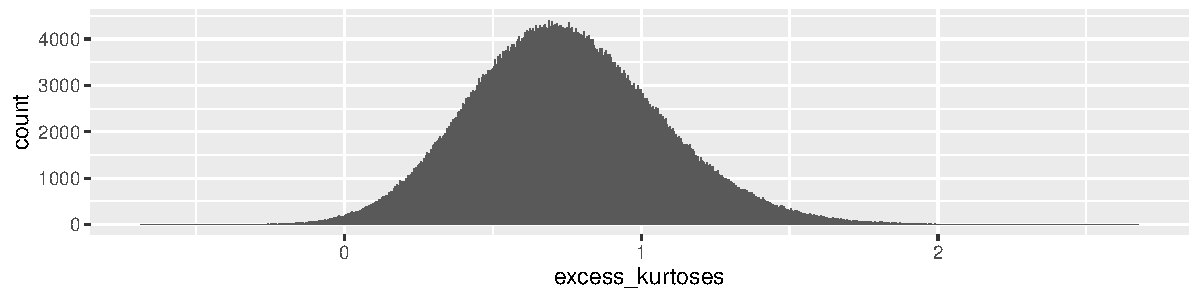
\includegraphics[width=7in]{boot}
\end{figure}


\vspace{-0.9cm}
\benum\truefalsesubquestionwithpoints{9} 
\begin{enumerate}[(a)]
\item We do not really need to use the bootstrap test as the sampling distribution of $\hat{\kappa}^{MM}_0$ can be derived analytically
\item A 95\% bootstrap confidence interval will be approximately between -1 and 3
\item A 95\% bootstrap confidence interval will be approximately between 0.2 and 1.4
\item The null hypothesis is rejected
\item The data seems to suggest the normal model is not a good model for daily percentage returns from the S\&P 500 in the past year
\item $B=1,000,000$ seems to be sufficient to construct CI's and run hypothesis tests
\item $\hat{\kappa}^{MM}_0$ may be biased
\item If $\hat{\kappa}^{MM}_0$ were to be biased, the test is still valid regardless of the bias
\item If $\hat{\kappa}^{MM}_0$ were to be biased, the bias could be fixed by increasing $n$
\end{enumerate}
\eenum\instr\pagebreak


%%%%%%%%%%%%%%%%%%%%%%%%

\problem\timedsection{15} Assume a DGP of $\Xoneton \iid \normnot{0}{\theta}$. We wish to test $H_a: \theta \neq 1$ for the dataset 1.41, 1.44, 4.19, 5.12, 0.09, 8.62, 0.6, -8.88, 0.63, -8.57 at $\alpha = 5\%$ using the score test.

\vspace{-0.1cm}
\benum\truefalsesubquestionwithpoints{14} 
\begin{enumerate}[(a)]
\item The score test requires you to compute $\doublehat{\theta}^{MLE}$
\item $\mathcal{L}\parens{\theta; \Xoneton} = \displaystyle\prod_{i=1}^n \oneoversqrt{2\pi\theta} \exp{-\oneover{2\theta} X_i^2}$
\item $\ell\parens{\theta; \Xoneton} = \tothepow{2\pi\theta}{-n/2} \natlog{-\oneover{2\theta} X_i^2}$
\item $\ell'\parens{\theta; \Xoneton} = -\displaystyle\frac{n}{2\pi} -\displaystyle\frac{n}{2\theta} - \oneover{2\theta} \sum_{i=1}^nX_i^2$
\item $\ell'\parens{\theta; \Xoneton} =-\displaystyle\frac{n}{2\theta} + \oneover{2\theta^2} \sum_{i=1}^n X_i^2$
\item $\ell''\parens{\theta; \Xoneton} = \displaystyle\frac{n}{2\theta^2} - \oneover{\theta^3} \sum_{i=1}^n X_i^2$
\item $I(\theta) = \displaystyle\frac{n}{2\theta^2}$
\item $I(\theta) = -\displaystyle\frac{n}{2\theta^2}$
\item The score statistic is $\parens{-\displaystyle\frac{n}{2} + \half \sum_{i=1}^n X_i^2} \displaystyle\overn{\sqrt{2}}$
\item The score statistic is 0
\item The score statistic is 16.40 rounded to the two nearest digits 
\item The score statistic is 89.98 rounded to the two nearest digits
\item The null hypothesis is rejected
\item The p-value of the score test will be similar to the p-values of the likelihood ratio test and the wald test but may not be exactly equal
\end{enumerate}
\eenum\instr\pagebreak


\end{document}




